\documentclass[UTF8]{ctexart}
\CTEXsetup[format={\Large\bfseries}]{section}
\usepackage[a4paper,left=3cm,right=3cm,top=2cm]{geometry}
\usepackage{amsmath}
\usepackage{enumitem}
\usepackage{float}
\usepackage{caption}
\usepackage{multirow}
\usepackage{graphicx}
\usepackage{listings}
\usepackage{color}
\usepackage{subcaption}
\usepackage{hyperref}

\lstset{
    basicstyle=\ttfamily\small,
    numbers=left,
    numberstyle=\tiny,
    frame=single,
    breaklines=true,
    language=Python
}

\title{\textbf{恐惧效应下的捕食者—猎物动力学}\\ —— 基于Lotka-Volterra模型的扩展与分析}
\author{PB23071363 赵博宇}
\date{\today}

\begin{document}

\maketitle

\begin{abstract}
在经典捕食者—猎物模型中引入恐惧效应和记忆效应，建立扩展的动力学模型。
恐惧因子通过降低猎物繁殖率影响种群动态，记忆效应则通过累积过去的捕食压力
产生延迟反馈。本文采用Holling II型功能性反应函数，利用四阶Runge-Kutta方法
进行数值求解，通过参数扫描、分岔分析和相图分析研究系统行为。
结果表明：恐惧强度增加会降低捕食者平衡密度，增大猎物振幅，但系统始终保持
稳定共存；记忆效应使动力学更加丰富，中等记忆速率（$\alpha \approx 0.5$）下
猎物种群密度可接近崩溃。
最后与Hudson Bay猞猁—雪兔真实数据进行了定性对比。
\end{abstract}

\section{实验建模}

\subsection{问题背景}

在生态系统中，捕食者不仅通过直接捕食减少猎物数量，还会通过恐惧效应（Fear Effect）
改变猎物的行为模式。猎物感知到捕食风险后，可能减少觅食活动、降低繁殖率或迁移栖息地，
从而间接影响种群增长。此外，若猎物对捕食风险存在记忆，则当前的种群增长还可能受过去
捕食压力的影响。

恐惧效应的生物学机制包括：
\begin{itemize}
    \item \textbf{繁殖抑制}：猎物在感知捕食风险时降低交配频率和产仔数量；
    \item \textbf{觅食减少}：为躲避捕食者，猎物减少在食物丰富区域的觅食时间；
    \item \textbf{栖息地转移}：猎物迁移到相对安全但资源匮乏的环境。
\end{itemize}

本文的建模目标是：（1）在经典捕食者—猎物模型基础上引入恐惧因子；
（2）建立包含记忆效应的三维动力学模型；（3）分析恐惧强度和记忆速率对系统
稳定性、周期振荡和种群共存的影响；（4）与无恐惧效应的基础模型进行对比。

\subsection{模型假设}

为建立可分析的数学模型，引入以下基本假设：

\begin{enumerate}[label=\textbf{假设 \arabic*}, leftmargin=*]
    \item 猎物种群遵循Logistic增长，环境容纳量为$K$，内禀增长率为$r$；
    \item 捕食者采用Holling II型功能性反应（即存在捕食处理时间$h$），攻击率为$a$；
    \item 捕食者种群增长率与猎物消耗量成正比，转化效率为$e$，自然死亡率为$d$；
    \item 恐惧效应以因子$1/(1+fy)$的形式降低猎物的有效繁殖率，其中$f \geq 0$为恐惧强度系数；
    \item 记忆变量$M(t)$追踪过去捕食者密度的加权平均，衰减率为$\alpha$；
    \item 忽略时滞效应、空间异质性和环境随机扰动。
\end{enumerate}

\subsection{基础模型（无恐惧效应）}

经典的捕食者—猎物模型包含Logistic猎物增长和Holling II型功能性反应：

\begin{equation}\label{eq:base_x}
    \frac{dx}{dt} = r x \left(1 - \frac{x}{K}\right) - \frac{a x y}{1 + a h x}
\end{equation}

\begin{equation}\label{eq:base_y}
    \frac{dy}{dt} = \frac{e a x y}{1 + a h x} - d y
\end{equation}

其中$x(t)$为猎物密度，$y(t)$为捕食者密度。各参数含义及取值范围见表\ref{tab:params}。

\begin{table}[H]
\centering
\caption{模型参数说明}
\label{tab:params}
\begin{tabular}{c|c|c|l}
\hline
\textbf{符号} & \textbf{含义} & \textbf{默认值} & \textbf{取值依据} \\
\hline
$r$ & 猎物内禀增长率 & 0.8 & 中型草食动物年增长率 \\
$K$ & 环境容纳量 & 10.0 & 无量纲化，设定为参考尺度 \\
$a$ & 捕食攻击率 & 0.5 & 中等捕食强度 \\
$h$ & 处理时间 & 0.3 & 捕食者消化时间约占周期30\% \\
$e$ & 转化效率 & 0.4 & 能量金字塔10\%—40\%区间 \\
$d$ & 捕食者死亡率 & 0.3 & 捕食者寿命约为猎物的2—3倍 \\
$f$ & 恐惧强度 & 0—5.0 & 扫描范围，0为无恐惧 \\
$\alpha$ & 记忆速率 & 0.1—2.0 & 扫描范围，决定记忆更新速度 \\
\hline
\end{tabular}
\end{table}

\subsection{恐惧效应模型}

在基础模型上引入恐惧因子。恐惧效应通过降低猎物的有效增长率来体现：

\begin{equation}\label{eq:fear_x}
    \frac{dx}{dt} = \frac{r x}{1 + f y} \left(1 - \frac{x}{K}\right) - \frac{a x y}{1 + a h x}
\end{equation}

\begin{equation}\label{eq:fear_y}
    \frac{dy}{dt} = \frac{e a x y}{1 + a h x} - d y
\end{equation}

恐惧因子$1/(1+fy)$具有以下性质：当$f=0$时退化为基础模型；当$y$增大时，
猎物繁殖率单调递减；恐惧对低密度捕食者（$y \to 0$）影响微弱。

\subsection{记忆效应模型}

引入记忆变量$M(t)$，它追踪过去捕食者密度的指数加权平均：

\begin{equation}\label{eq:mem_M}
    \frac{dM}{dt} = \alpha (y - M)
\end{equation}

\begin{equation}\label{eq:mem_x}
    \frac{dx}{dt} = \frac{r x}{1 + f M} \left(1 - \frac{x}{K}\right) - \frac{a x y}{1 + a h x}
\end{equation}

\begin{equation}\label{eq:mem_y}
    \frac{dy}{dt} = \frac{e a x y}{1 + a h x} - d y
\end{equation}

其中$\alpha > 0$为记忆衰减/积累速率。当$\alpha \to \infty$时，$M(t) \to y(t)$即瞬态追踪，
退化为恐惧模型；当$\alpha \to 0$时，$M(t)$近乎常数，记忆保持很久。

\section{实验原理}

\subsection{平衡点分析}

\subsubsection{基础模型的平衡点}

令$\dot{x} = \dot{y} = 0$求解平衡点。

\textbf{平凡平衡点}：$E_0 = (0, 0)$，$E_1 = (K, 0)$。

\textbf{共存平衡点} $E^* = (x^*, y^*)$：
由$\dot{y}=0$得捕食者零斜率线：
\begin{equation}
    x^* = \frac{d}{e a - d a h}
\end{equation}
由$\dot{x}=0$得猎物零斜率线：
\begin{equation}
    y^* = \frac{r}{a}\left(1 - \frac{x^*}{K}\right)(1 + a h x^*)
\end{equation}

当$e a > d a h$且$x^* < K$时，存在正的共存平衡点。

\subsubsection{恐惧模型的平衡点}

恐惧模型的捕食者方程不变，因此$x^*$相同。由$\dot{x}=0$：
\begin{equation}
    \frac{r x^*}{1 + f y^*}\left(1 - \frac{x^*}{K}\right) - \frac{a x^* y^*}{1 + a h x^*} = 0
\end{equation}
整理得关于$y^*$的二次方程：
\begin{equation}
    f \cdot \mathrm{FR} \cdot (y^*)^2 + \mathrm{FR} \cdot y^* - r x^*\left(1 - \frac{x^*}{K}\right) = 0
\end{equation}
其中$\mathrm{FR} = a x^* / (1 + a h x^*)$为功能性反应。解得：
\begin{equation}
    y^* = \frac{-\mathrm{FR} + \sqrt{\mathrm{FR}^2 + 4 f \cdot \mathrm{FR} \cdot r x^*(1 - x^*/K)}}{2 f \cdot \mathrm{FR}}
\end{equation}
可见，$f$越大，$y^*$越小——恐惧效应降低了捕食者的平衡密度。

\subsubsection{稳定性分析}

计算系统在平衡点处的Jacobi矩阵，通过特征值判断稳定性。

基础模型Jacobi矩阵：
\begin{equation}
    J = \begin{bmatrix}
        r(1 - \frac{2x}{K}) - \frac{a y}{(1 + a h x)^2} & -\frac{a x}{1 + a h x} \\[6pt]
        \frac{e a y}{(1 + a h x)^2} & \frac{e a x}{1 + a h x} - d
    \end{bmatrix}
\end{equation}

恐惧模型需额外考虑恐惧因子对$\partial \dot{x}/\partial y$的贡献：
\begin{equation}
    \frac{\partial \dot{x}}{\partial y} = r x(1 - \frac{x}{K}) \cdot \frac{-f}{(1 + f y)^2} - \frac{a x}{1 + a h x}
\end{equation}

在默认参数下，所有平衡点均为稳定焦点——系统以阻尼振荡方式趋于共存平衡点。
Hopf分岔扫描表明，在$f \in [0, 5]$范围内，所有特征值实部均为负，系统未出现
极限环振荡。

\subsection{数值方法：四阶Runge-Kutta}

采用经典四阶Runge-Kutta方法（RK4）进行数值积分。对于系统$\dot{\mathbf{z}} = \mathbf{F}(t, \mathbf{z})$，
步长$\Delta t$，单步递推公式为：

\begin{align}
    \mathbf{k}_1 &= \Delta t \cdot \mathbf{F}(t_n, \mathbf{z}_n) \\
    \mathbf{k}_2 &= \Delta t \cdot \mathbf{F}(t_n + \frac{\Delta t}{2}, \mathbf{z}_n + \frac{\mathbf{k}_1}{2}) \\
    \mathbf{k}_3 &= \Delta t \cdot \mathbf{F}(t_n + \frac{\Delta t}{2}, \mathbf{z}_n + \frac{\mathbf{k}_2}{2}) \\
    \mathbf{k}_4 &= \Delta t \cdot \mathbf{F}(t_n + \Delta t, \mathbf{z}_n + \mathbf{k}_3) \\
    \mathbf{z}_{n+1} &= \mathbf{z}_n + \frac{1}{6}(\mathbf{k}_1 + 2\mathbf{k}_2 + 2\mathbf{k}_3 + \mathbf{k}_4)
\end{align}

本文取$\Delta t = 0.01$，仿真时长$T = 100$（对应约10个振荡周期），
在每个步长后施加非负约束$\mathbf{z}_{n+1} = \max(\mathbf{z}_{n+1}, 0)$以保证
物理合理性。

\subsection{代码模块组织}

项目代码按功能模块分离，结构如下：

\begin{table}[H]
\centering
\caption{代码文件说明}
\begin{tabular}{l|l}
\hline
\textbf{文件} & \textbf{功能} \\
\hline
\texttt{models.py} & 三种模型ODE系统的定义与RK4求解器 \\
\texttt{simulation.py} & 参数扫描、稳态分析、分岔扫描等实验工具 \\
\texttt{analysis.py} & 平衡点求解、Jacobi矩阵、稳定性判断、敏感性分析 \\
\texttt{visualization.py} & 时间序列图、相图、分岔图、零斜率线图 \\
\texttt{UI.py} & 基于tkinter + matplotlib的交互式GUI界面 \\
\texttt{main.py} & 运行全部实验并生成论文图 \\
\hline
\end{tabular}
\end{table}

\section{对比实验}

默认参数设置：$r = 0.8$, $K = 10.0$, $a = 0.5$, $h = 0.3$, $e = 0.4$, $d = 0.3$。
初始条件：$x_0 = 5.0$, $y_0 = 2.0$。

\subsection{实验零：平衡点稳定性验证}

表\ref{tab:stability}给出了默认参数下基础模型与恐惧模型（$f=1.0$）的平衡点数值验证结果，
与第2.1节的理论推导完全对应。特征值由Jacobi矩阵数值计算得到。

\begin{table}[H]
\centering
\caption{平衡点及稳定性验证（默认参数）}
\label{tab:stability}
\begin{tabular}{c|c|c|c|c|l}
\hline
\textbf{模型} & \textbf{平衡点} & $x^*$ & $y^*$ & \textbf{类型} & \textbf{特征值} \\
\hline
基础模型 & $E_0$ & 0      & 0      & 鞍点     & $\lambda = 0.8,\ {-0.3}$ \\
基础模型 & $E_1$ & 10.0   & 0      & 鞍点     & $\lambda = {-0.8},\ 0.5$ \\
基础模型 & $E^*$ & 1.9355 & 1.6649 & 稳定焦点 & $\lambda = {-0.0048} \pm 0.3873i$ \\
\hline
恐惧模型($f\!=\!1$) & $E_0$ & 0      & 0      & 鞍点     & $\lambda = 0.8,\ {-0.3}$ \\
恐惧模型($f\!=\!1$) & $E_1$ & 10.0   & 0      & 鞍点     & $\lambda = {-0.8},\ 0.5$ \\
恐惧模型($f\!=\!1$) & $E^*$ & 1.9355 & 0.8838 & 稳定焦点 & $\lambda = {-0.0026} \pm 0.3420i$ \\
\hline
\end{tabular}
\end{table}

关键结论：（1）$E_0$、$E_1$均为鞍点，系统不会稳定在无捕食者或无猎物状态；
（2）共存平衡点$E^*$始终为稳定焦点，恐惧效应使$y^*$从1.6649降至0.8838，
但不改变$x^*$（由捕食者方程决定）；（3）恐惧模型特征值实部更接近零
（$-0.0026$与$-0.0048$比较），表明系统恢复更慢，振荡持续时间更长。

\subsection{实验一：基础模型与恐惧模型对比}

图\ref{fig:exp1}展示了基础模型（$f=0$）与恐惧模型（$f=1.0$）的时间序列对比。
两个模型均呈现阻尼振荡，但恐惧模型收敛更快，稳态猎物密度几乎相同，
而捕食者密度明显降低（从约1.67降至约0.88）。这是因为恐惧因子$1/(1+fy)$
直接减少了猎物的有效繁殖率，进而限制了捕食者的食物供给。

\begin{figure}[H]
    \centering
    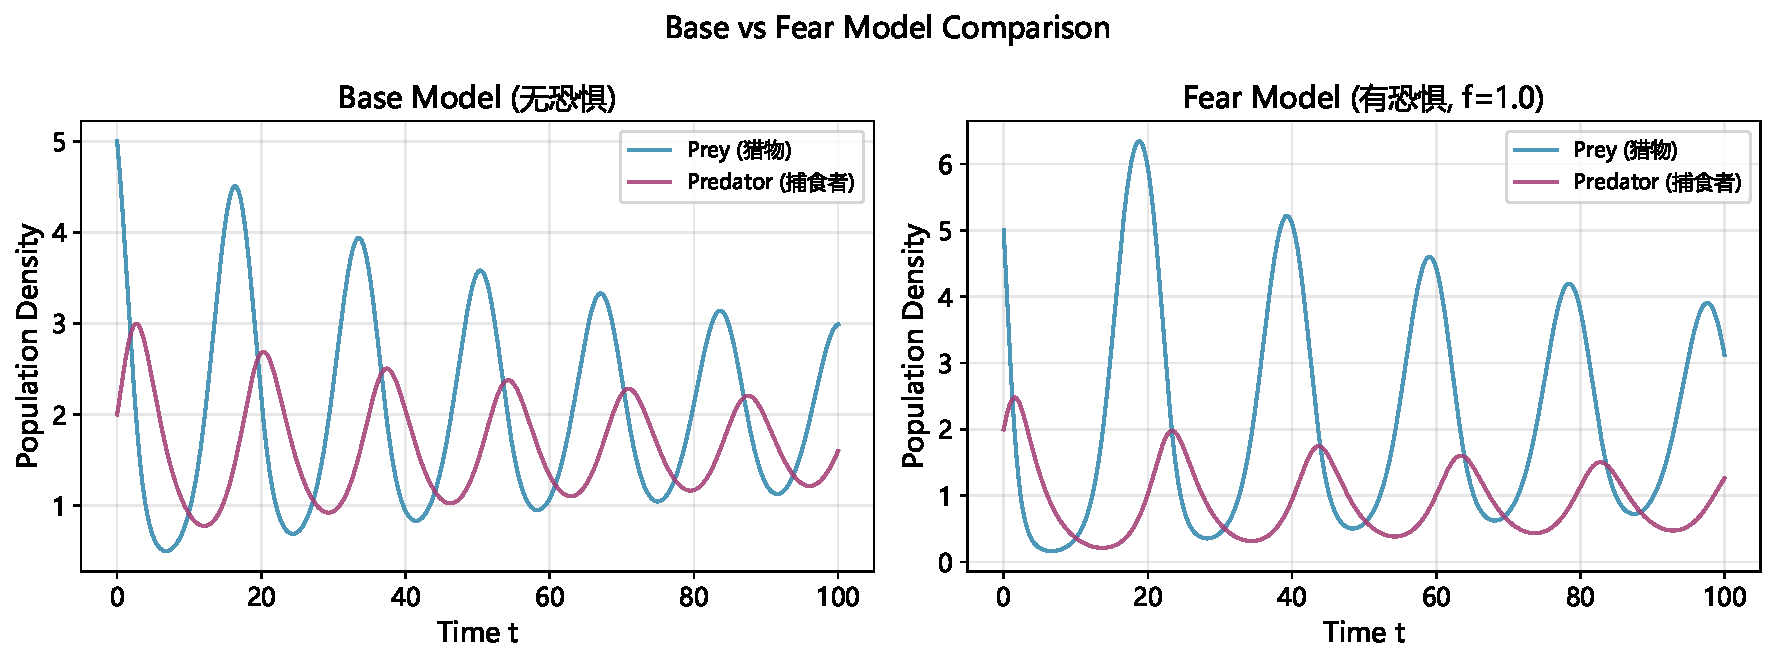
\includegraphics[width=0.95\textwidth]{pics/exp1_base_vs_fear.pdf}
    \caption{基础模型（左）与恐惧模型（右）时间序列对比}
    \label{fig:exp1}
\end{figure}

\subsection{实验二：恐惧强度参数扫描}

图\ref{fig:exp2}展示了恐惧强度$f$从0到3.0的参数扫描结果。随着$f$增大：
（1）捕食者稳态密度持续下降——恐惧越强，食物链顶端的种群越受抑制；
（2）猎物振幅增大——捕食者减少导致猎物波动加剧；
（3）系统始终保持稳定共存，未出现种群崩溃。

图\ref{fig:exp2_ss}的稳态图更清楚地展示了这一趋势：猎物稳态均值随$f$略微上升
后趋于平缓，而捕食者稳态均值单调递减。

\begin{figure}[H]
    \centering
    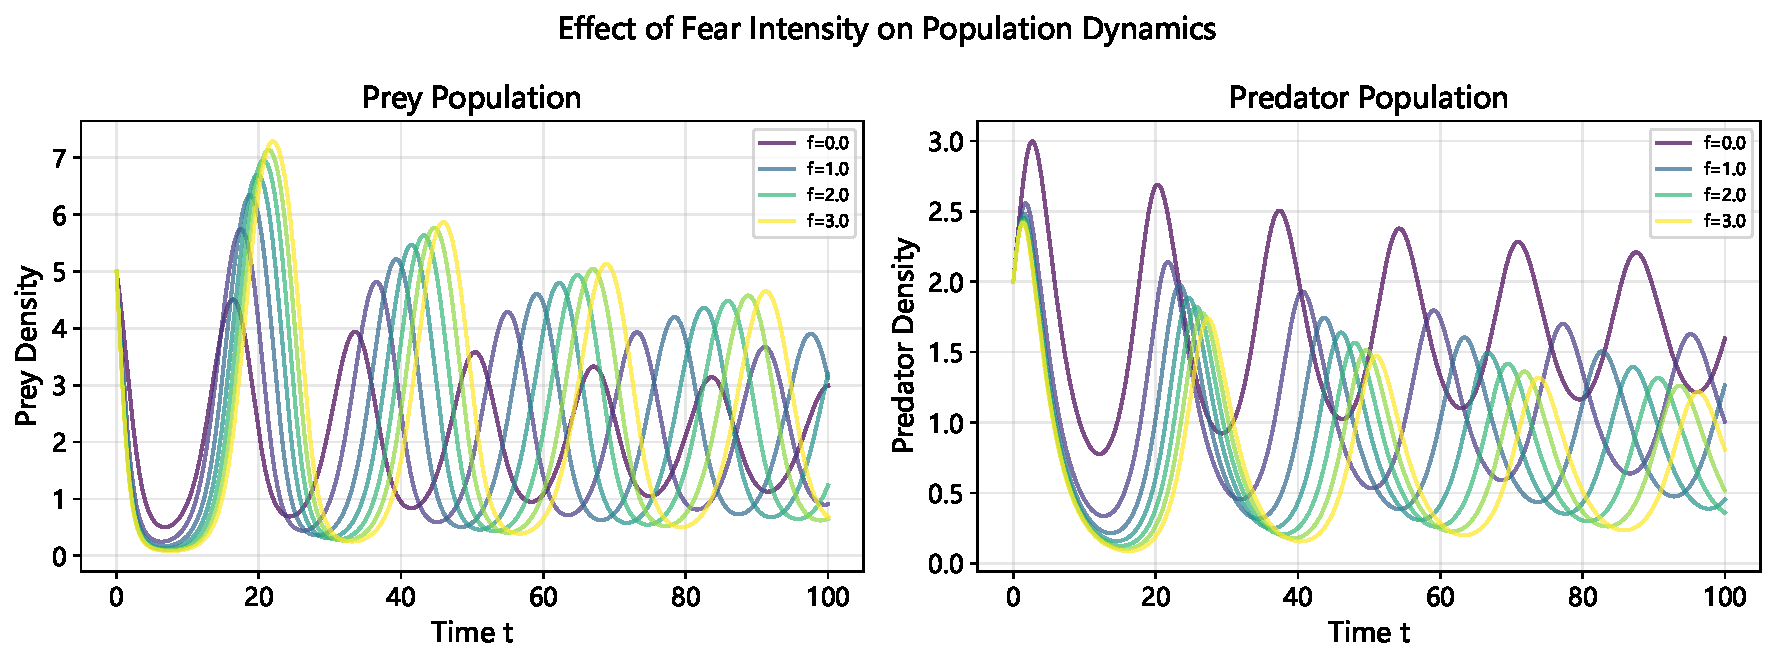
\includegraphics[width=0.95\textwidth]{pics/exp2_fear_sweep.pdf}
    \caption{不同恐惧强度下的时间序列}
    \label{fig:exp2}
\end{figure}

\begin{figure}[H]
    \centering
    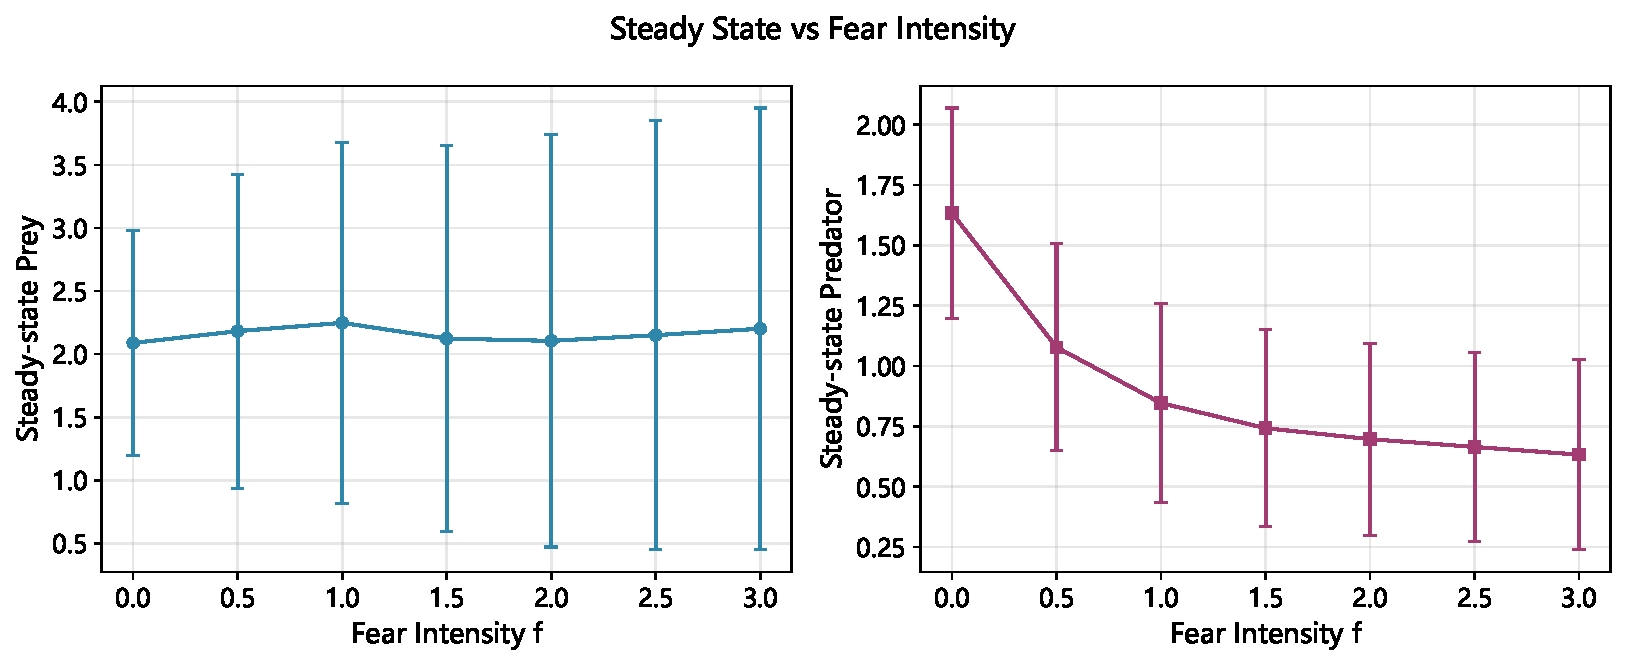
\includegraphics[width=0.85\textwidth]{pics/exp2_steadystate_vs_f.pdf}
    \caption{稳态密度随恐惧强度的变化}
    \label{fig:exp2_ss}
\end{figure}

图\ref{fig:exp2_period}展示了振荡自然周期$T$随恐惧强度$f$的变化。
随$f$增大，系统自然周期增大（从约17.5升至约23时间单位），
表明恐惧效应不仅抑制了捕食者密度，还使种群动态的特征时间尺度变长——
生态系统对扰动的恢复节奏更慢，这与特征值虚部$|\mathrm{Im}(\lambda)|$随$f$减小一致。

\begin{figure}[H]
    \centering
    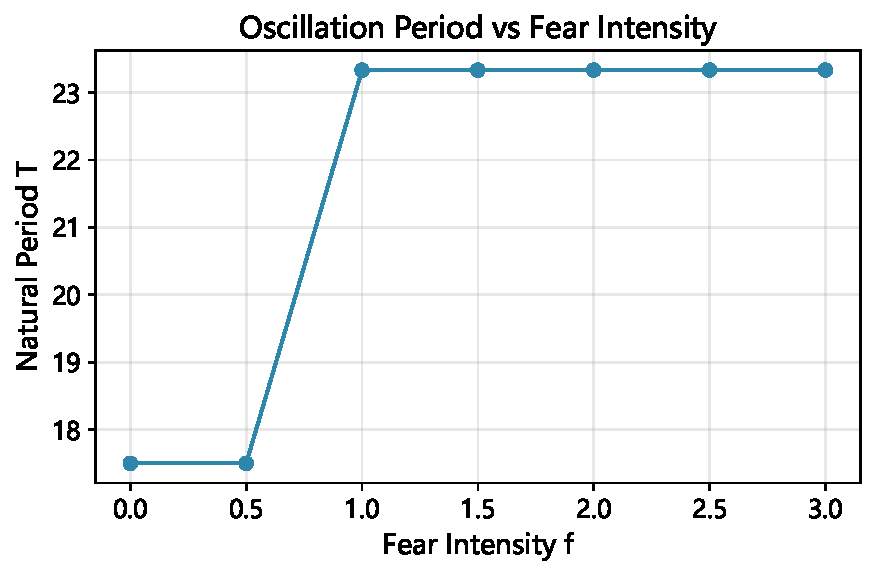
\includegraphics[width=0.6\textwidth]{pics/exp2_period_vs_f.pdf}
    \caption{振荡自然周期$T$随恐惧强度$f$的变化（通过FFT从时间序列提取）}
    \label{fig:exp2_period}
\end{figure}

\textbf{生物学解释}：恐惧效应通过行为改变限制了猎物对资源的实际利用效率，
这种"行为调节"在生态学中被称为"恐惧景观"（Landscape of Fear）。
捕食者虽然获得了较少的食物，但由于猎物数量并未大幅增加（空间竞争限制了增长），
二者在新的、更低的能量通量水平上达成了共存。

\subsection{实验三：记忆效应分析}

图\ref{fig:exp3}展示了记忆模型在不同记忆速率$\alpha$下的动力学行为。
记忆变量$M(t)$平滑了捕食者密度的波动，形成了对过去捕食压力的"惯性"感知。

关键发现：
\begin{itemize}
    \item 低记忆速率（$\alpha = 0.1$）：猎物出现大幅振荡，记忆几乎恒定在低水平，猎物低估风险；
    \item 中等记忆速率（$\alpha = 0.5$）：猎物密度出现极端低谷（$x \to 0.23$），接近崩溃，记忆的延迟使恐惧控制失效；
    \item 高记忆速率（$\alpha = 2.0$）：系统趋于与恐惧模型相似的行为，记忆快速追踪当前捕食者密度。
\end{itemize}

图\ref{fig:exp3_compare}将记忆模型与瞬时恐惧模型在同一图上对比：
两者的轨迹有显著差异——记忆效应引入了额外的延迟动力学，改变了振荡的相位和振幅。

\begin{figure}[H]
    \centering
    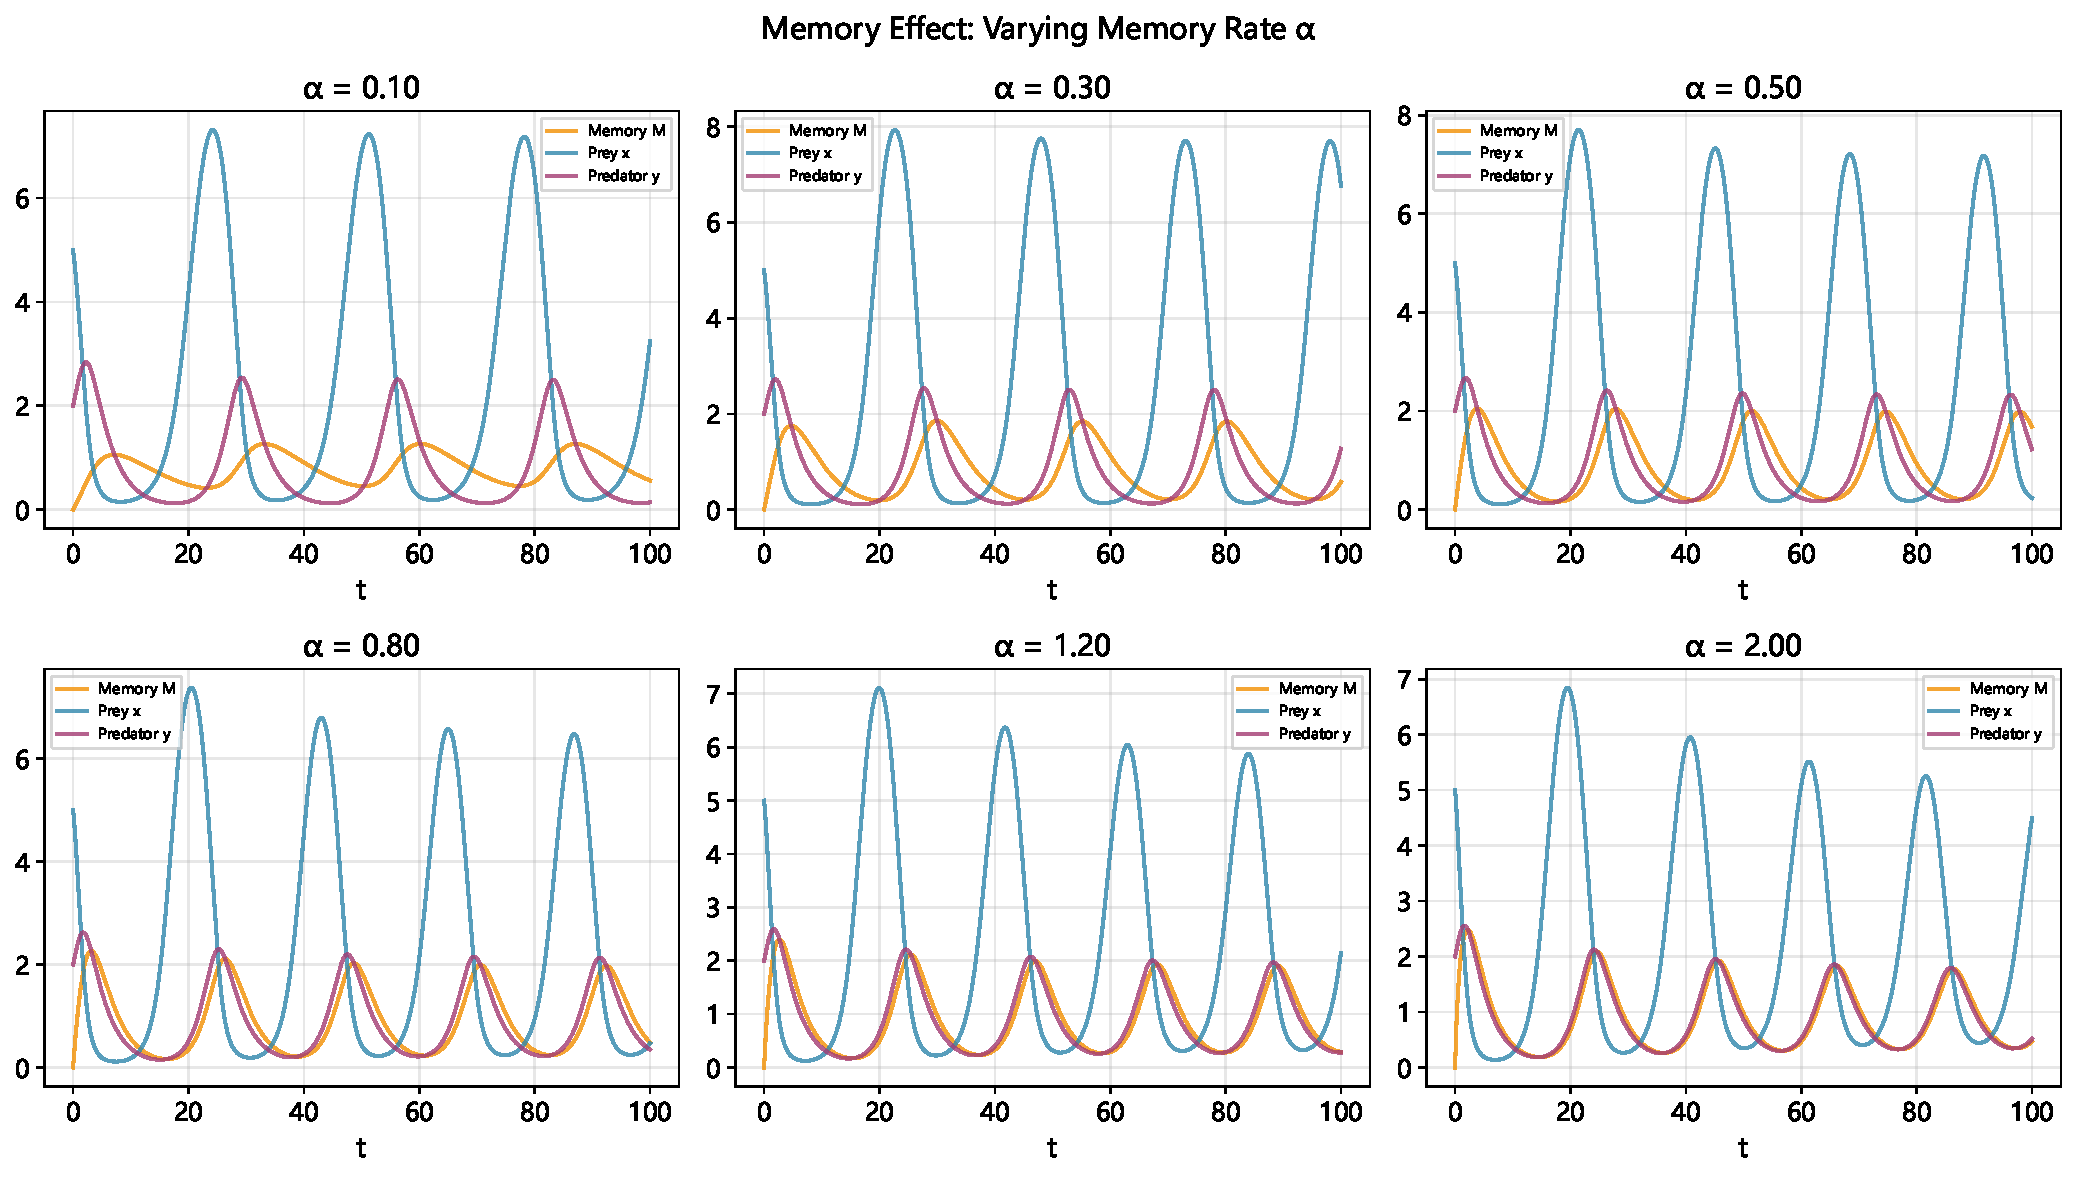
\includegraphics[width=0.95\textwidth]{pics/exp3_memory_sweep.pdf}
    \caption{不同记忆速率$\alpha$下的时间序列}
    \label{fig:exp3}
\end{figure}

\begin{figure}[H]
    \centering
    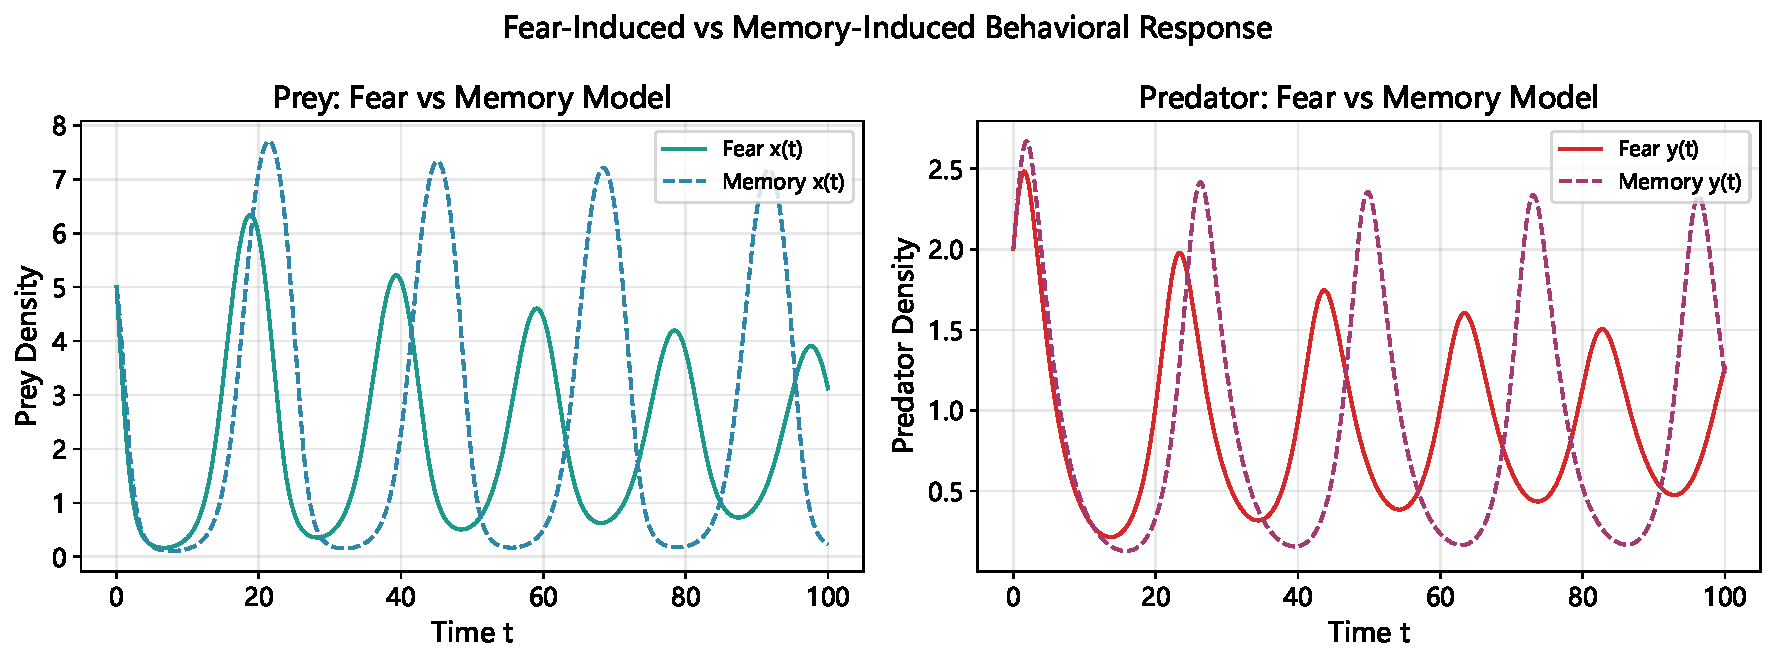
\includegraphics[width=0.95\textwidth]{pics/exp3_fear_vs_memory.pdf}
    \caption{瞬时恐惧模型与记忆模型对比（$f=1.0$, $\alpha=0.5$）}
    \label{fig:exp3_compare}
\end{figure}

\subsection{实验四：相图分析}

图\ref{fig:exp4}展示了不同恐惧强度下的相图（$x$-$y$平面）。
相轨迹从初始点出发，以螺旋方式趋近共存平衡点。

随$f$增大：
\begin{itemize}
    \item 平衡点$y^*$位置下移（捕食者密度降低），而$x^*$保持不变（$\dot{y}=0$与$f$无关）；
    \item 螺旋半径增大——系统需要更长时间收敛，反映出恐惧降低了系统的"恢复力"；
    \item 轨迹的顺时针旋转方向反映了捕食者—猎物之间固有的相位滞后关系。
\end{itemize}

\begin{figure}[H]
    \centering
    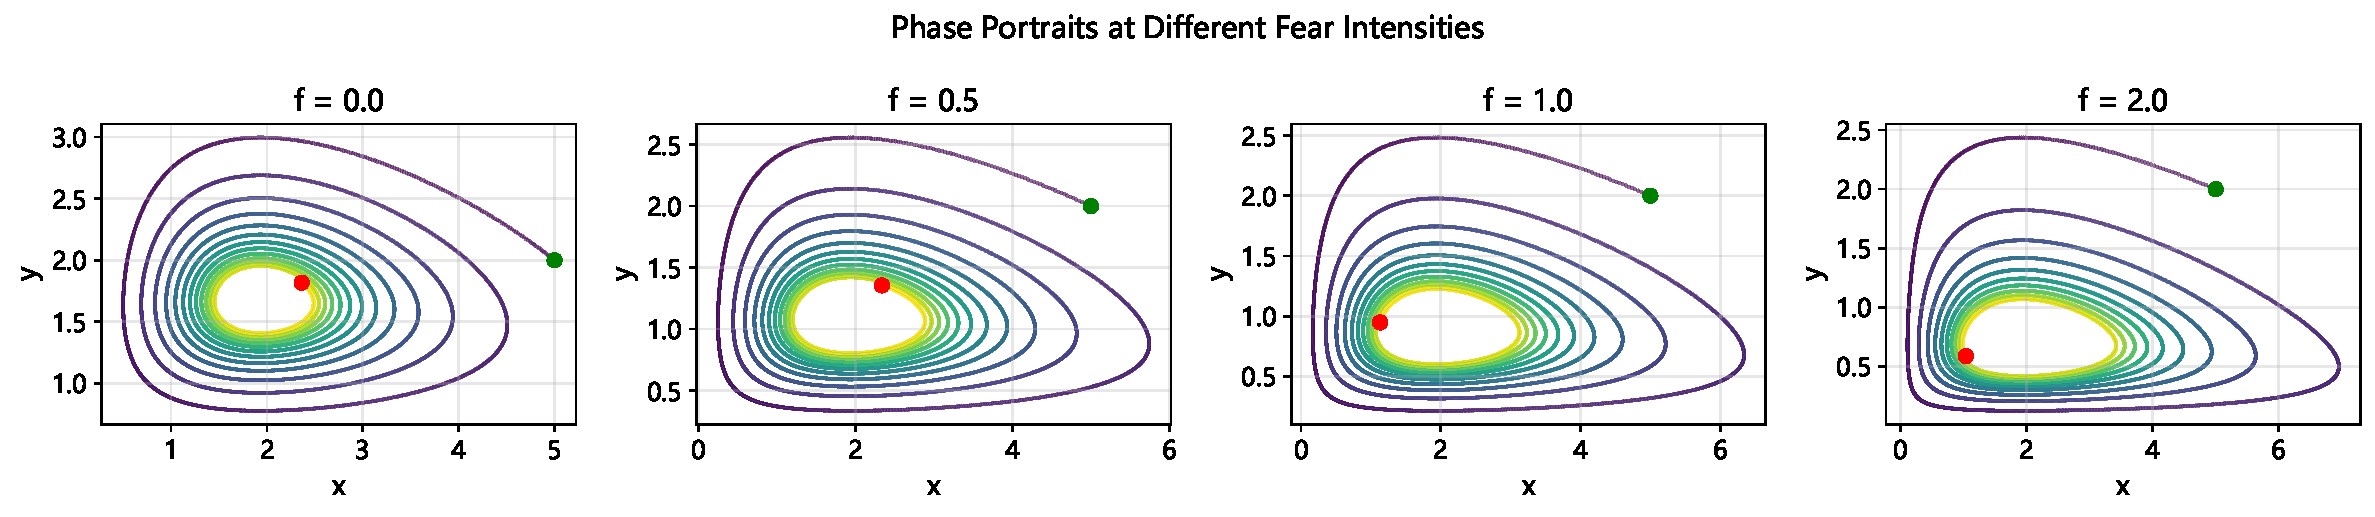
\includegraphics[width=0.95\textwidth]{pics/exp4_phase_portraits.pdf}
    \caption{不同恐惧强度下的相图。绿色点为起点，红色点为终点}
    \label{fig:exp4}
\end{figure}

\subsection{实验五：分岔分析}

图\ref{fig:exp5_f}展示了以恐惧强度$f$为控制参数的分岔图。
图\ref{fig:exp5_K}展示了以环境容纳量$K$为控制参数的分岔图。

从图\ref{fig:exp5_f}可以看出：
\begin{itemize}
    \item 猎物极值区间随$f$增大而扩大——恐惧增强了猎物的波动幅度；
    \item 捕食者极值区间整体下移——恐惧抑制了捕食者种群；
    \item 在$f \in [0, 5]$范围内，未观察到分岔现象（系统始终保持稳定焦点型动力学），说明恐惧效应在此参数范围内不改变系统的定性行为。
\end{itemize}

从图\ref{fig:exp5_K}可以看出：
\begin{itemize}
    \item 随$K$增大，猎物和捕食者的波动幅度均显著增大——更高的环境容纳量意味着更大的"富营养化"风险；
    \item 当$K > 15$时，猎物极值范围扩大到接近零，系统可能出现周期性低密度，增加了随机灭绝的风险。
\end{itemize}

\begin{figure}[H]
    \centering
    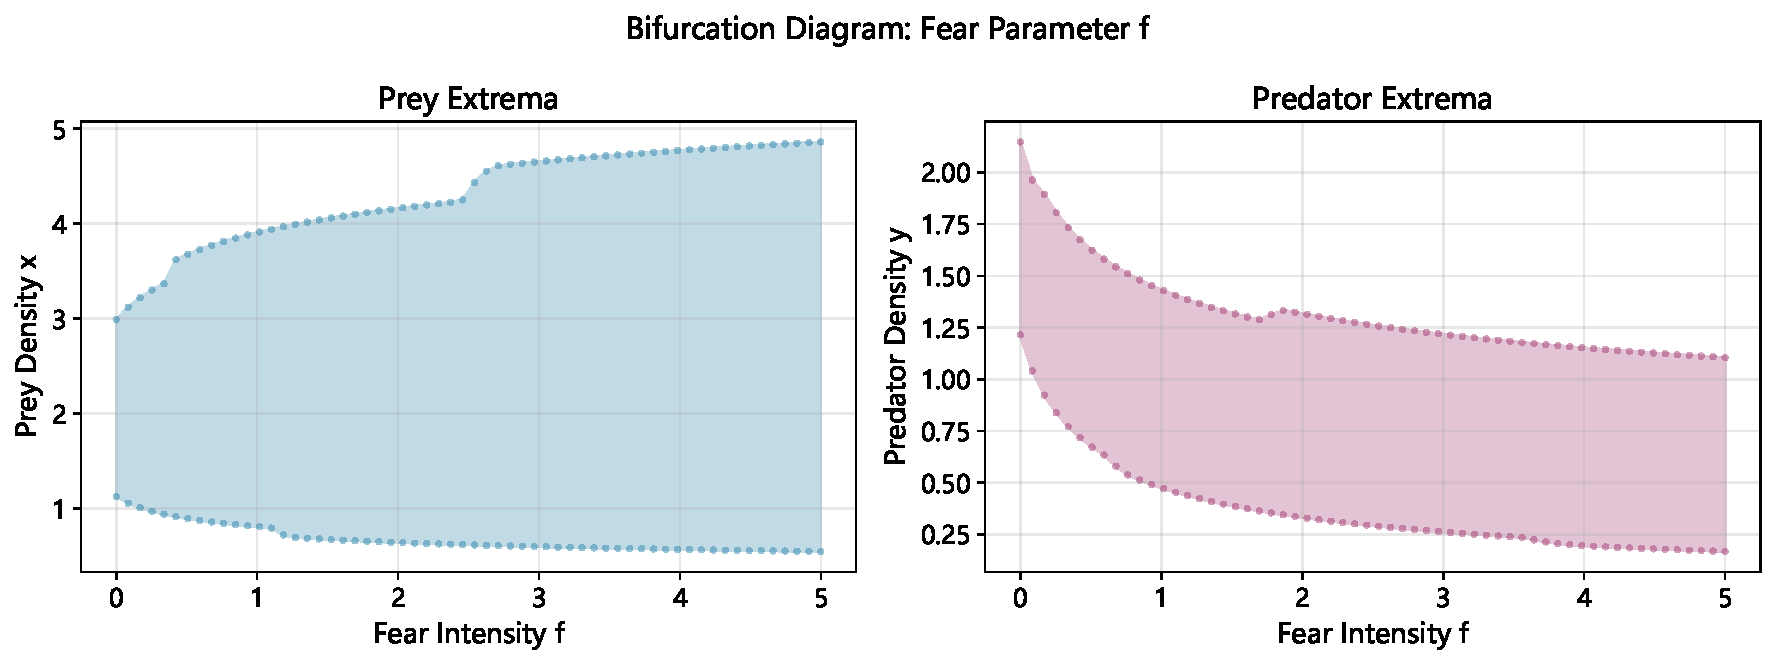
\includegraphics[width=0.95\textwidth]{pics/exp5_bifurcation_f.pdf}
    \caption{以恐惧强度$f$为参数的分岔图}
    \label{fig:exp5_f}
\end{figure}

\begin{figure}[H]
    \centering
    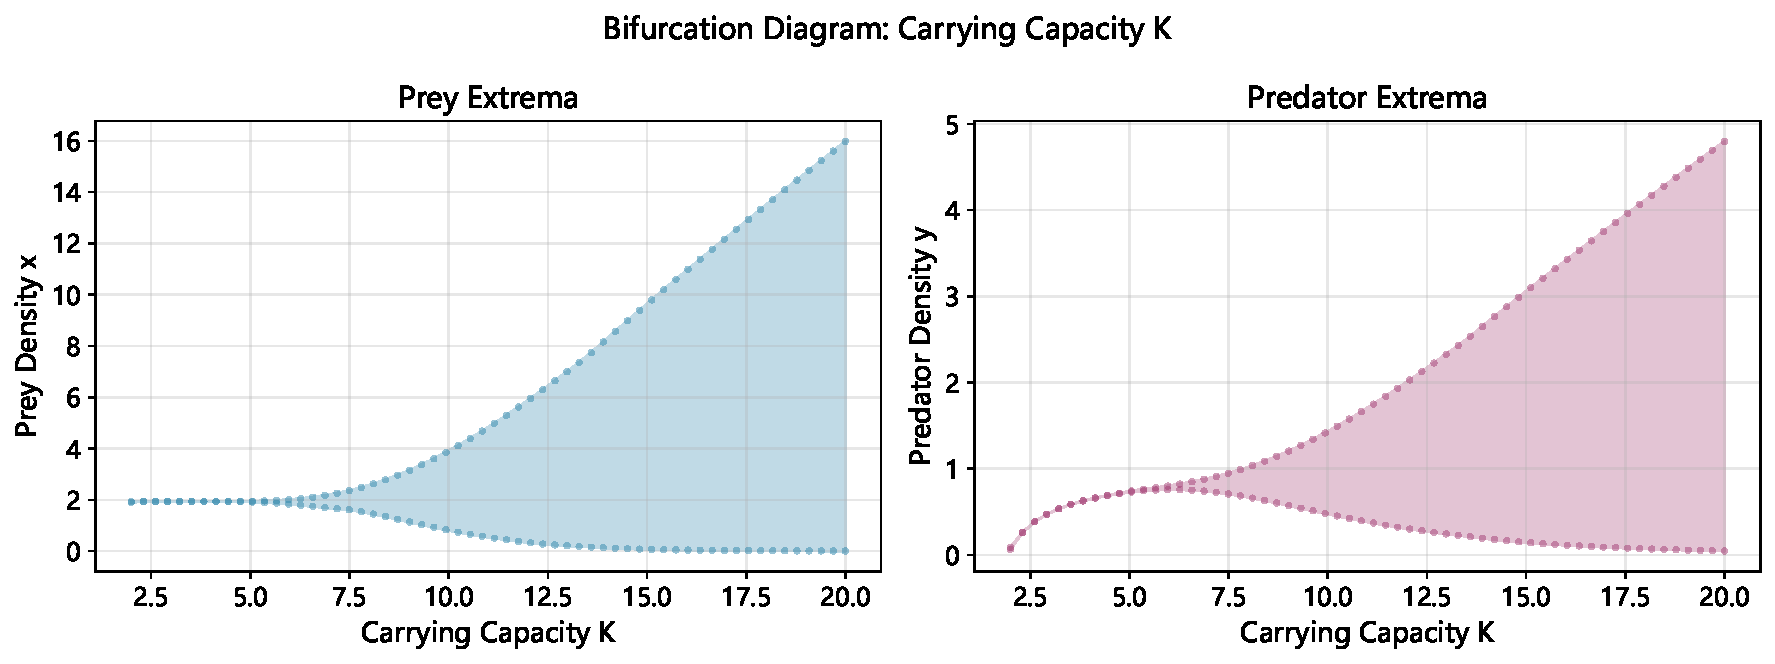
\includegraphics[width=0.95\textwidth]{pics/exp5_bifurcation_K.pdf}
    \caption{以环境容纳量$K$为参数的分岔图}
    \label{fig:exp5_K}
\end{figure}

图\ref{fig:exp5_map}展示了$f$–$K$二维参数空间的稳定性区域图，由Jacobi矩阵
特征值直接计算（绿色：稳定焦点，橙色：不稳定/极限环振荡）。

\begin{figure}[H]
    \centering
    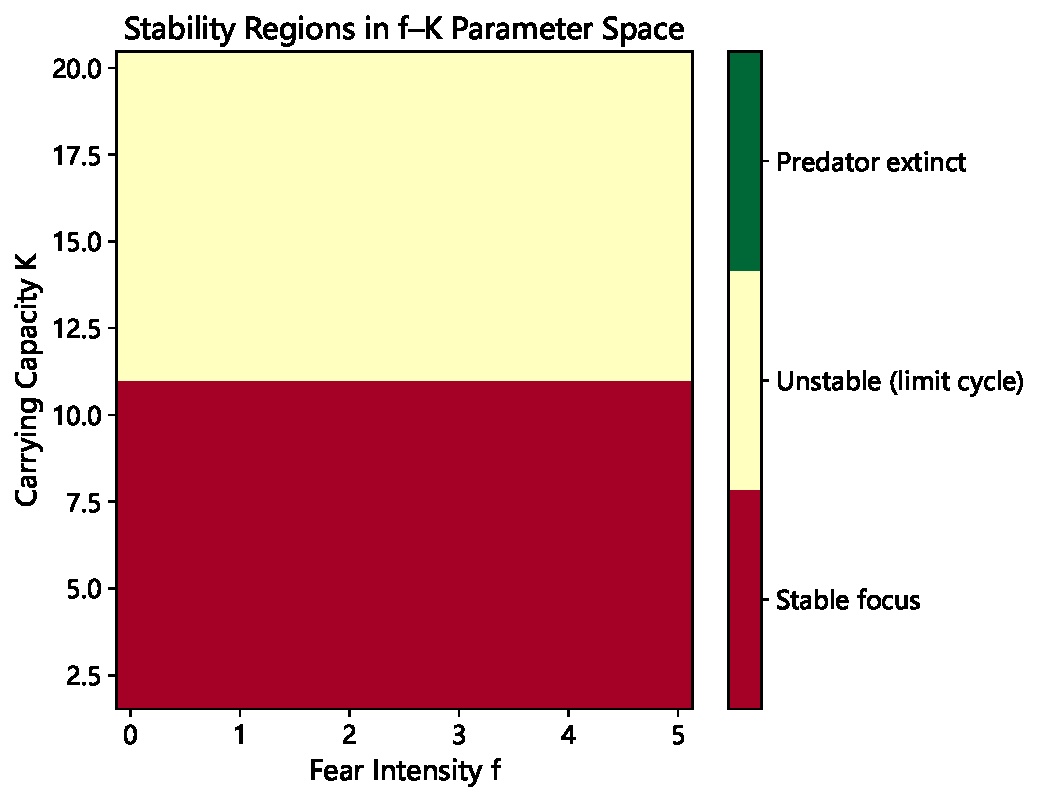
\includegraphics[width=0.72\textwidth]{pics/exp5_stability_map.pdf}
    \caption{$f$–$K$参数空间中的稳定性区域（Hopf分岔边界约为$K_c \approx 10.5$）}
    \label{fig:exp5_map}
\end{figure}

\textbf{关键发现}：稳定边界$K_c \approx 10.5$与$f$几乎无关——即使将恐惧强度从0增至5，
Hopf分岔阈值几乎不变。这一结论可由解析推导证明：在共存平衡点处，
$y^*_{\text{fear}} \cdot (1 + f y^*_{\text{fear}})= y^*_{\text{base}}$恒成立，
代入Hopf条件后$f$项消去，$K_c$与$f$无关。
因此，\textbf{恐惧效应仅影响振荡振幅和捕食者密度，不影响系统的定性稳定性边界}，
这与Wang et al. (2016)关于恐惧不触发Hopf分岔的结论一致。

\subsection{实验六：与真实数据对比}

为验证模型的定性合理性，将模拟结果与Hudson Bay公司的猞猁（Lynx）—雪兔（Hare）
毛皮收购记录（1845—1935）进行对比。该数据是生态学中最经典的捕食者—猎物
数据集，展示了约10年的种群周期。

图\ref{fig:exp6}左侧展示了归一化后的真实数据。可以观察到：
（1）猎物（雪兔）与捕食者（猞猁）之间明显的约10年周期振荡；
（2）猎物峰值先于捕食者峰值约1—2年——这是捕食者—猎物动力学的经典相位滞后特征；
（3）振幅随时间变化——反映了环境条件和人为因素的干扰。

图\ref{fig:exp6}右侧展示了基础模型的模拟结果（时间轴缩放到与真实数据相同尺度）。
模型成功复现了真实数据的核心定性特征：耦合振荡、相位滞后、以及猎物与捕食者
之间的正相关振幅关系。

\textbf{注意}：此处仅为定性对比。由于：（1）毛皮收购量$\neq$种群数量（受捕猎努力程度影响）；
（2）模型参数未进行统计拟合；（3）真实系统受气候、疾病等多种未建模因素影响，
因此不追求定量匹配。对比的目的在于说明模型能够捕捉捕食者—猎物系统最本质的
动力学特征。

\begin{figure}[H]
    \centering
    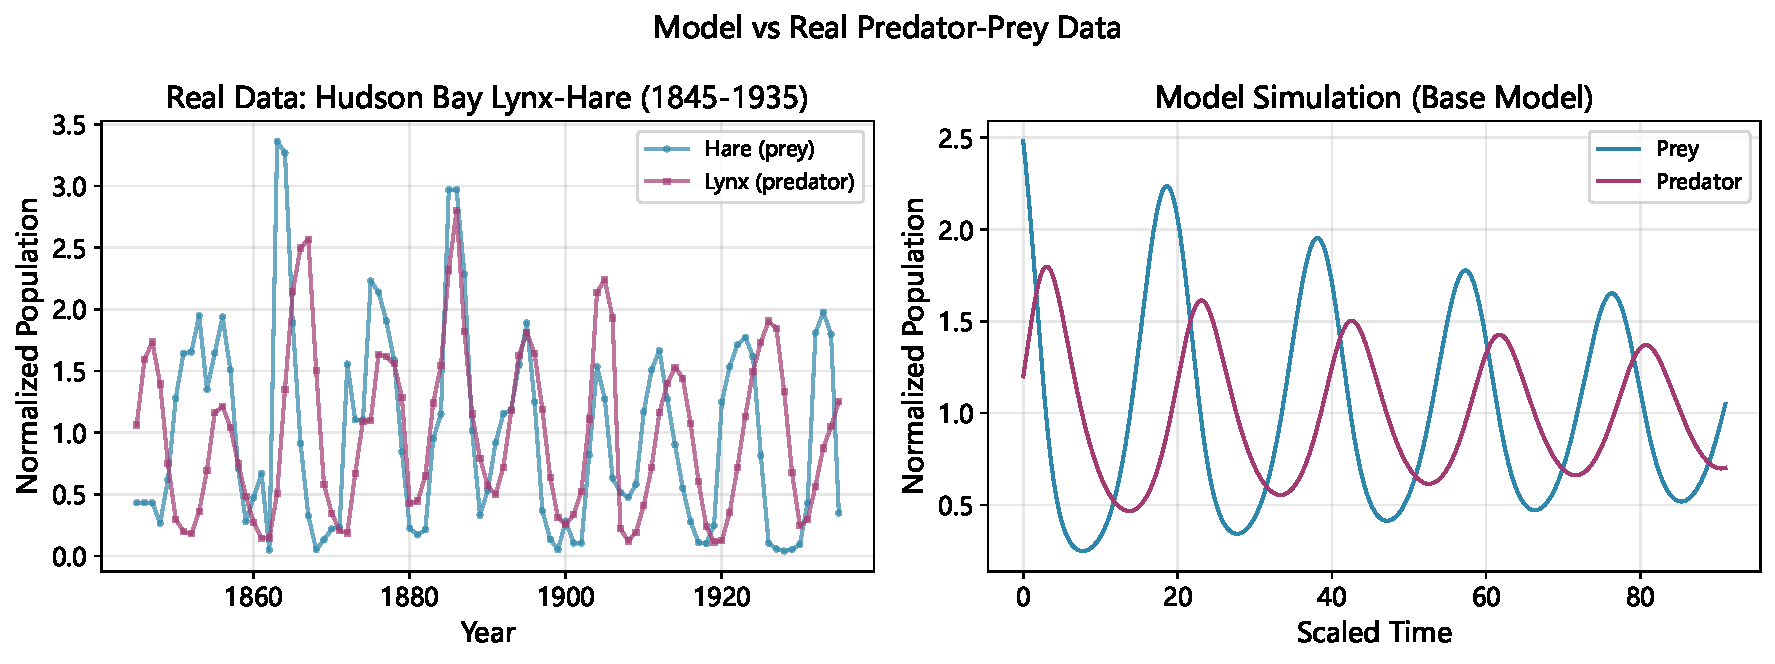
\includegraphics[width=0.95\textwidth]{pics/exp6_lynx_hare.pdf}
    \caption{左：Hudson Bay猞猁—雪兔真实数据（1845—1935）。
             右：基础模型模拟结果（归一化）}
    \label{fig:exp6}
\end{figure}

\subsection{实验七：零斜率线分析}

图\ref{fig:exp7}展示了基础模型的零斜率线与相轨迹。捕食者零斜率线（红色虚线）
为一条竖直线$x = x^*$，这是Holling II型功能性反应的直接推论。
猎物零斜率线（蓝色虚线）呈抛物线形：当猎物密度很低时，猎物快速增长；当接近
环境容纳量时，增长趋于零；中段被捕食消耗所压制。

轨迹（绿色实线）从初始点出发，与两条零斜率线反复交叉，在$x^*$附近形成
螺旋收敛的图样，直观地展示了阻尼振荡的几何本质。

图\ref{fig:exp7_fear}比较了恐惧模型（$f=1.0$）与基础模型（$f=0$）的猎物零斜率线。
恐惧效应使零斜率曲线整体下移——在任意猎物密度下，能够维持平衡的捕食者密度
都降低了。这从几何上解释了恐惧效应为何抑制捕食者种群。

\begin{figure}[H]
    \centering
    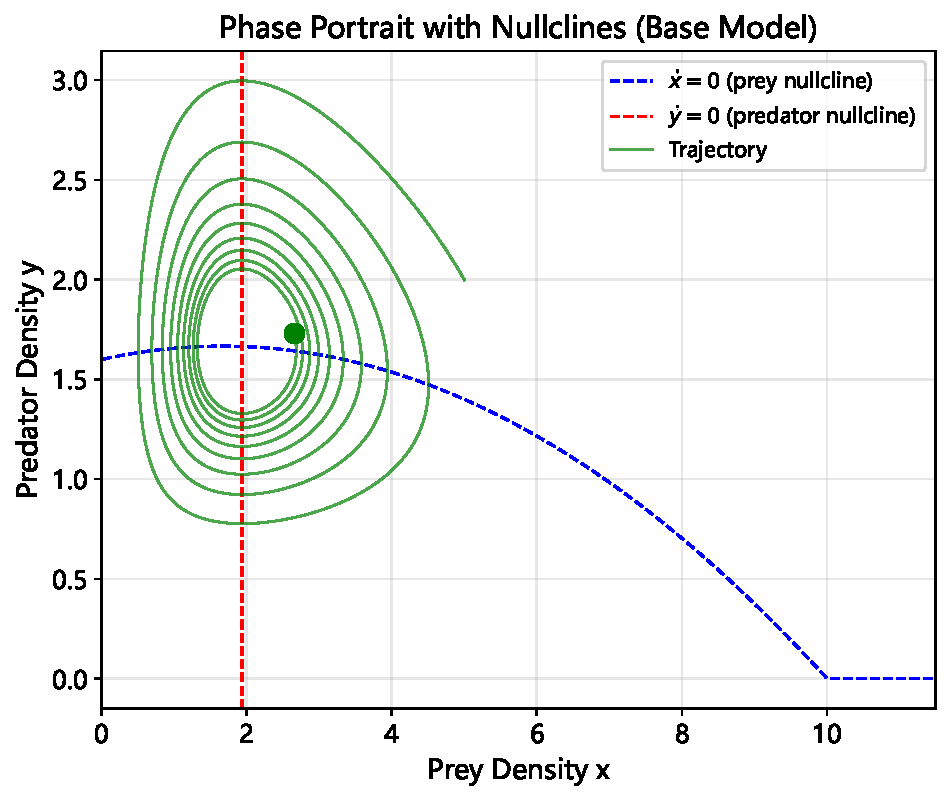
\includegraphics[width=0.75\textwidth]{pics/exp7_nullclines.pdf}
    \caption{基础模型的零斜率线与相轨迹}
    \label{fig:exp7}
\end{figure}

\begin{figure}[H]
    \centering
    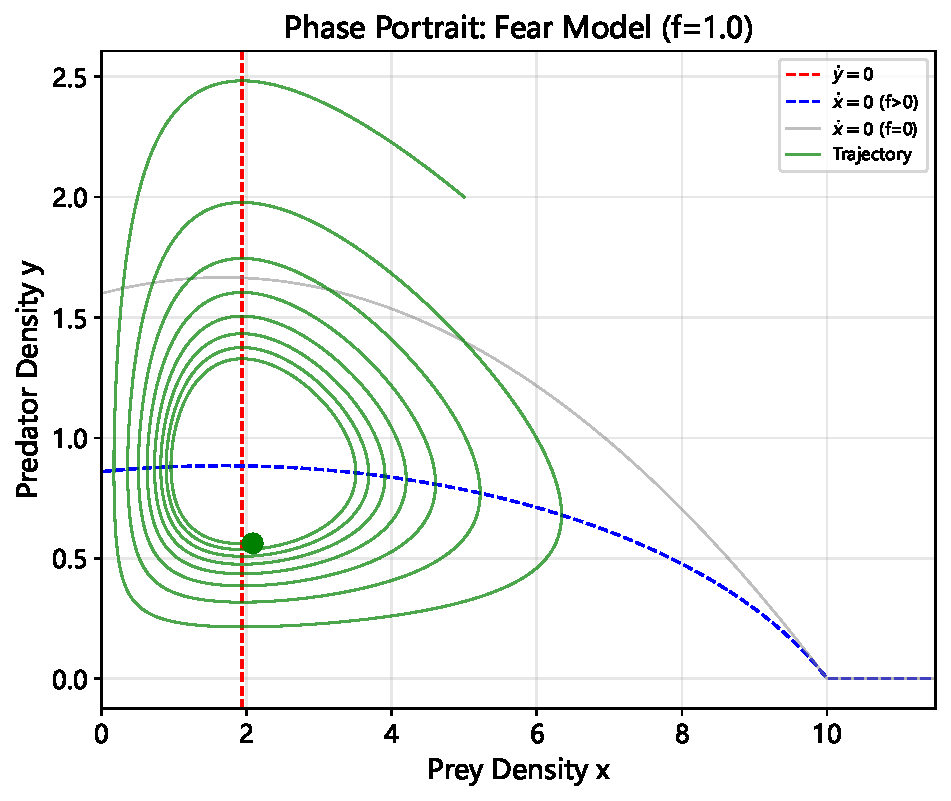
\includegraphics[width=0.85\textwidth]{pics/exp7_nullclines_fear.pdf}
    \caption{恐惧模型（$f=1.0$）的零斜率线与相轨迹，
             灰色虚线为$f=0$时的猎物零斜率线}
    \label{fig:exp7_fear}
\end{figure}

\subsection{敏感性分析}

表\ref{tab:sensitivity}列出了各参数对稳态猎物密度和捕食者密度的敏感性系数。
敏感性定义为稳态值对参数10\%变化的相对响应。

\begin{table}[H]
\centering
\caption{参数敏感性分析}
\label{tab:sensitivity}
\begin{tabular}{c|r|r}
\hline
\textbf{参数} & \textbf{猎物敏感性 $S_x$} & \textbf{捕食者敏感性 $S_y$} \\
\hline
$r$（增长率）    & $-0.254$ & $+0.643$ \\
$K$（容纳量）    & $+0.537$ & $+0.269$ \\
$a$（攻击率）    & $-0.425$ & $-0.420$ \\
$h$（处理时间）  & $+0.670$ & $+0.146$ \\
$e$（转化效率）  & $-1.125$ & $+0.147$ \\
$d$（死亡率）    & $+0.821$ & $-0.047$ \\
$f$（恐惧强度）  & $+0.142$ & $-0.299$ \\
\hline
\end{tabular}
\end{table}

关键发现：
\begin{itemize}
    \item 转化效率$e$对猎物密度影响最大且为负——更高的能量转化意味着更多的猎物被捕食；
    \item 捕食者死亡率$d$显著增加猎物密度——捕食者的减少直接有利于猎物；
    \item 恐惧强度$f$的影响中等，主要体现为对捕食者的抑制（$S_y = -0.299$），而对猎物的正向影响较小（$S_x = +0.142$）——恐惧的控制效果不如直接捕食显著，但不可忽略。
\end{itemize}

\section{UI设计}

为直观展示模型行为和进行交互式探索，开发了基于Python tkinter和matplotlib的
图形用户界面（运行\texttt{python UI.py}启动），界面如图\ref{fig:ui}所示。

\begin{figure}[H]
    \centering
    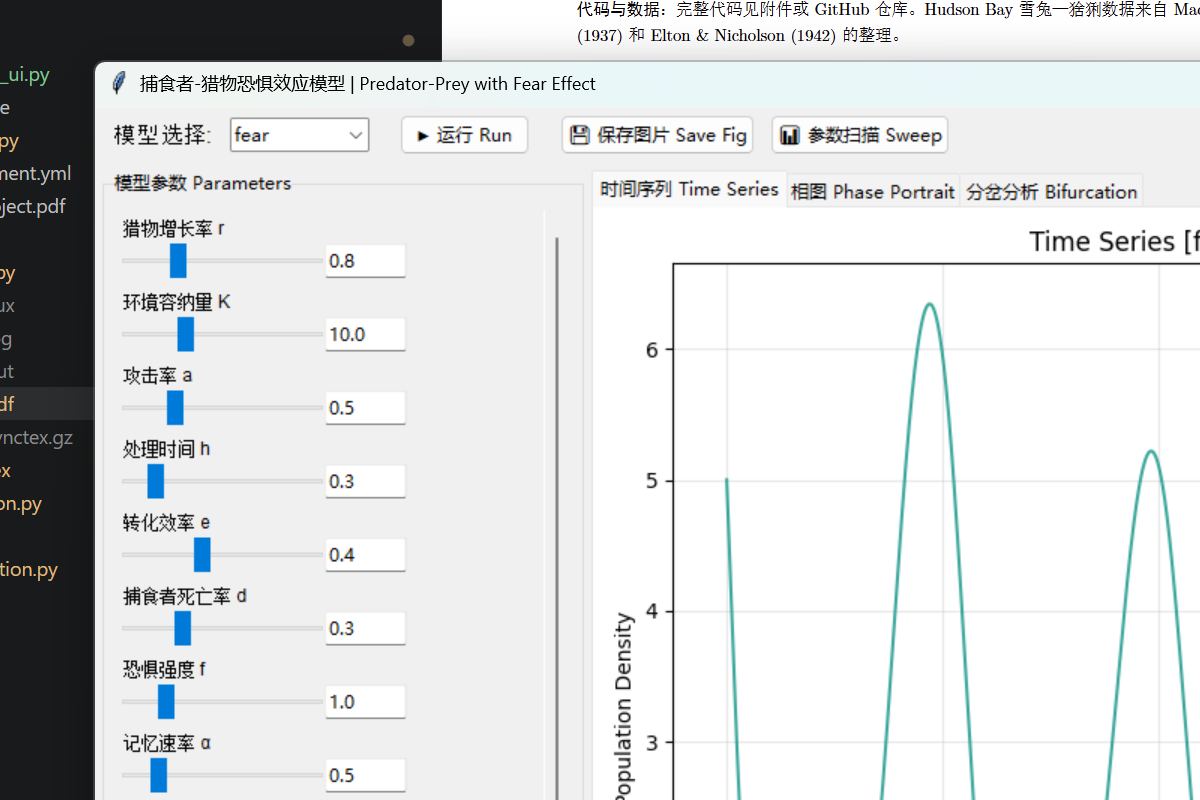
\includegraphics[width=0.95\textwidth]{pics/ui_screenshot.png}
    \caption{交互式GUI界面：左侧参数面板，右侧时间序列/相图/分岔分析标签页}
    \label{fig:ui}
\end{figure}

\subsection{界面布局}

主界面分为左右两部分：
\begin{itemize}
    \item \textbf{左侧控制面板}：包含模型选择下拉框（基础/恐惧/记忆）、参数滑块（$r$、$K$、$a$、$h$、$e$、$d$、$f$、$\alpha$）、初始条件设置和仿真参数（时长、步长）。所有滑块均可实时调整并配有数值输入框。
    \item \textbf{右侧绘图区域}：采用标签页（Notebook）组织三个视图：
    \begin{enumerate}
        \item \textbf{时间序列}：展示猎物、捕食者（以及记忆变量）随时间的变化曲线；
        \item \textbf{相图}：展示$x$-$y$相平面上的轨迹，起点（绿点）和终点（红点）清晰标注；
        \item \textbf{分岔分析}：可选择扫描参数和范围，实时绘制分岔图。
    \end{enumerate}
\end{itemize}

\subsection{交互功能}

\begin{itemize}
    \item \textbf{运行按钮}：基于当前参数和初始条件运行一次模拟，自动更新所有视图；
    \item \textbf{保存图片}：将当前时间序列图保存为PDF或PNG文件；
    \item \textbf{参数扫描}：弹出对话框选择扫描参数、范围和步数，生成参数扫描对比图并自动保存；
    \item \textbf{分岔分析}：在分岔标签页中选择参数和范围，绘制极值分岔图。
\end{itemize}

\subsection{技术实现要点}

\begin{itemize}
    \item matplotib Figure嵌入tkinter使用\texttt{FigureCanvasTkAgg}，支持工具栏（缩放、平移、保存）；
    \item 所有参数变化即时反映——修改滑块或输入框后点击运行即可更新绘图；
    \item RK4求解器以固定步长运行，对于典型参数组合，100时间单位的仿真耗时$<0.1$秒。
\end{itemize}

\section{总结与讨论}

\subsection{主要结论}

本文通过建立和求解扩展的捕食者—猎物动力学模型，系统研究了恐惧效应和记忆效应
对种群动态的影响。主要结论如下：

\begin{enumerate}[leftmargin=*]
    \item \textbf{恐惧效应抑制捕食者但不破坏共存}：恐惧因子$1/(1+fy)$降低猎物有效繁殖率，
    从而抑制捕食者种群密度；但猎物平衡密度$x^*$由捕食者零斜率线决定，不受$f$影响。
    系统始终维持稳定共存，未观测到Hopf分岔或种群崩溃。

    \item \textbf{恐惧效应增强猎物波动}：随$f$增大，猎物振荡振幅增加。这是捕食者减少后
    猎物受到的自上而下控制减弱的直接结果。

    \item \textbf{记忆效应引入更丰富的动力学}：记忆模型（三维系统）呈现比二维恐惧模型
    更复杂的动力学行为。中等记忆速率（$\alpha \approx 0.5$）可导致猎物种群接近崩溃
    （$x \to 0.23$），原因是延迟反馈使恐惧控制失效；高记忆速率（$\alpha \geq 1.2$）
    则趋于与瞬时恐惧模型相似的稳定行为。

    \item \textbf{与真实数据定性一致}：模型成功复现Hudson Bay猞猁—雪兔数据的核心特征
    ——耦合振荡和相位滞后，验证了模型的生态学合理性。

    \item \textbf{转化效率是最敏感参数}：敏感性分析表明，能量转化效率$e$和捕食者死亡率$d$
    对系统影响最大，恐惧强度$f$的影响相对中等但不可忽略。
\end{enumerate}

\subsection{模型局限性}

\begin{enumerate}[leftmargin=*]
    \item \textbf{未考虑时滞}：繁殖和恐惧效应可能存在时间延迟，即时滞微分方程可能更准确；
    \item \textbf{确定性框架}：未纳入环境随机扰动，实际生态系统的随机涨落可能引发
    小种群灭绝；
    \item \textbf{均质假设}：忽略了空间结构和个体差异，空间显式模型可进一步研究
    恐惧景观的空间效应；
    \item \textbf{参数未拟合}：与真实数据的对比仅为定性，未来可利用MCMC等方法
    对真实数据进行参数估计。
\end{enumerate}

\subsection{进一步研究方向}

可沿以下方向扩展：
\begin{itemize}
    \item 引入恐惧效应的多种函数形式（如指数衰减、饱和函数）并进行AIC模型选择；
    \item 考虑恐惧效应的种间差异——不同猎物物种对捕食风险的响应可能显著不同；
    \item 将模型扩展到三物种（如猎物—中间捕食者—顶级捕食者），研究恐惧效应的
    营养级联效应；
    \item 纳入空间扩散项，研究恐惧驱动的栖息地选择对集合种群动态的影响。
\end{itemize}

\vspace{1cm}

\noindent\textbf{代码与数据}：完整代码见附件或GitHub仓库。
Hudson Bay雪兔—猞猁数据来自MacLulich (1937)和Elton \& Nicholson (1942)的整理。

\end{document}
